\documentclass{article} % For LaTeX2e
\usepackage{nips15submit_e,times}
\usepackage{hyperref}
\usepackage{url}
\usepackage{graphicx}
\usepackage{amsfonts}
\usepackage{amssymb}
\usepackage{float}
\usepackage{listings}
\usepackage{xcolor}
\usepackage{amsmath}
%\documentstyle[nips14submit_09,times,art10]{article} % For LaTeX 2.09


\title{Problem Set 5 for Machine Learning 15 Fall}


\author{
Jingyuan Liu\\
AndrewId: jingyual\\
\texttt{jingyual@andrew.cmu.edu} \\
}


\newcommand{\fix}{\marginpar{FIX}}
\newcommand{\new}{\marginpar{NEW}}
\newcommand{\argmin}{\arg\!\min}
\newcommand{\norm}[1]{\left\lVert #1 \right\rVert}
\newcommand{\abs}[1]{\left\lvert #1 \right\rvert}
\newcommand{\inner}[1]{\left\langle #1 \right\rangle}


\nipsfinalcopy % Uncomment for camera-ready version


\begin{document}
\maketitle



\section{VC dimension}


\subsection{Show the VC dimension of linear classifier}
To prove that the linear classifier h with x in $ R^n $ has the VC dimension of
n + 1, we need to prove that $VCdim(h_n) >= n + 1$, and then prove that
$VCdim(h_n) <= n + 1$.

\textbf{(a). Prove $VCdim(h_n) >= n+1$}

First of all, we could use the Mathematical Induction to prove that $VCdim(H) >=
n+1$:

For n = 1, it is easy to get $VCdim(h_1) >= 2$

For n = 2, we could also get $VCdim(h_2) >= 3$, which could be proved using following figures:

\begin{figure}[!htbp]
\begin{center}
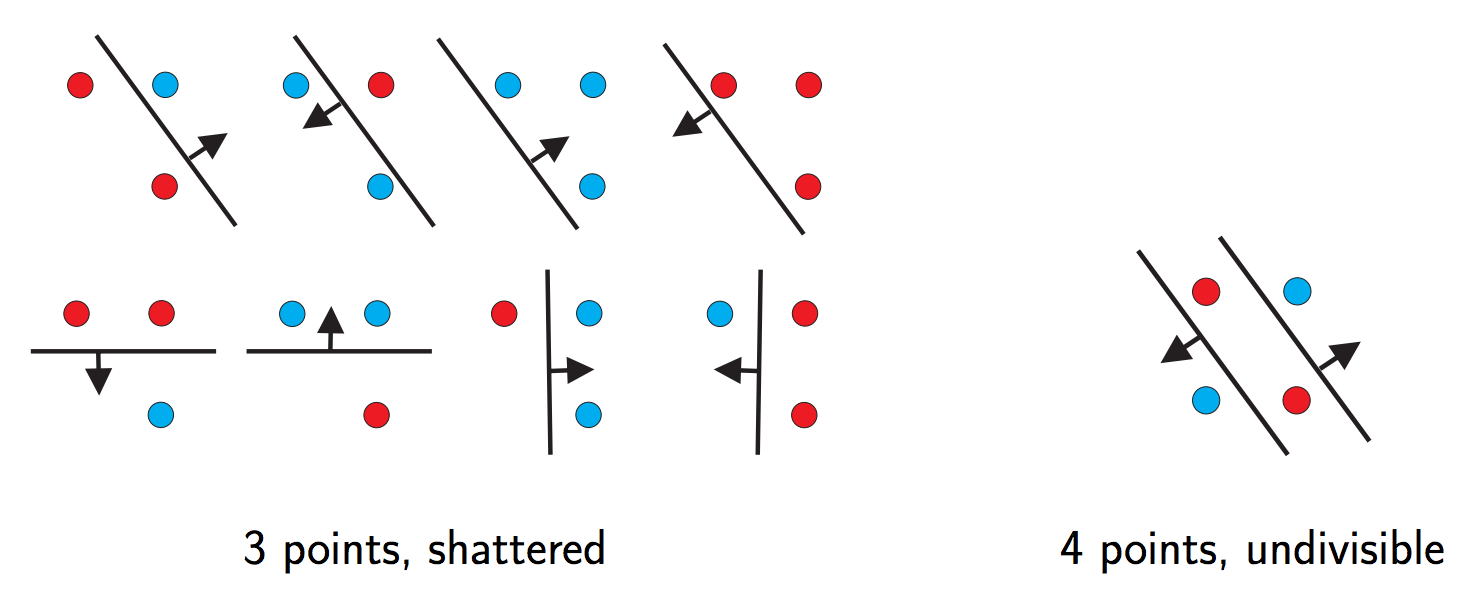
\includegraphics[width=80mm]{pic/q11.png}
\end{center}
\caption{The representation of $VCdim(h_2)$}
\end{figure}

For n = i, we assume that the $VCdim(h_i) >= i+1$. We could form a matrix of
(i+1)*(i+1),
with the rank of i+1, since the VCdim is i+1.

For n = i+1, we could form a matrix of (i+2)*(i+2), since the variable
x have one more independent dimension. Therefore, $VCdim(h_{i+1}) >= VCdim(h_i) + 1
>= i+2$.

Therefore, we have $VCdim(h_n) >= n+1$. We could use a more straight forward
detailed example to show that. Say we have n dimensions of the data, then we
could construct a dataset:

$1th$: \quad (1,0,0,...,0)

$2th$: \quad (0,1,0,...,0)

$ith$: \quad (0,0,...,i..,0)

$nth$: \quad (0,0,0,...,n)

$n+1th$: \quad (0,0,....,0)

For these dataset, we could see that for the ith data point, the ith dimension
is 1, otherwise 0. And for the n+1th data, all dimension are 0. In this case, we
could see that the linear classifier could shatter this dataset.

\textbf{(b). Prove $VCdim(h_n) <= n+1$}

Then we should prove that $VCdim(h_n) <= n+1$:

Suppose we could shatter n+2 points, then using the convex combinations of
points in C, we could seperate points into S1 and S2, that:

\begin{equation}
conv(s1) \cap conv(s2) \neq \emptyset
\end{equation}

However, if $VCdim(h_n) = n+2$, then we could spilt points to half space
contains s1 and the complement of the half space contains s2. This implies that
the both half space contains the convex hull of s1 and the complement of the
half space the contains the convex hull of s2. Thus, we get:

\begin{equation}
conv(s1) \cap conv(s2) = \emptyset
\end{equation}

These two observations are contradictory to each other. So we know that for the
n+2 points here, we could not use the linear classifier to shatter all of them.

\textbf{In conclusion}, we prove that $VCdim(h_n) >= n+1$ and $VCdim(h_n) <= n+1$ for the
linear classifier, then we have $VCdim(h_n) = n+1$


\subsection{Show the VC dimension of axis-aligned boxes}

Similarily, for this case, to prove that the axis-aligned boxes classifier h
with x in $ R^n $ has the VC dimension of 2n, we need to prove that
$VCdim(h_n) >= 2n$, and then prove that $VCdim(h_n) <= 2n$.

\textbf{(a). Prove $VCdim(h_n) >= 2n$}

First of all, we need to prove that for any case, $VCdim(h_n) >= 2n$, which
means if the x has n dimensions, we can use the axis-aligned boxes classifiers
to shatter 2n points.

Suppose we have n dimensions, then we can map all the x to a dimension i. In the
dimension i, we can have $x^i_{max}$ and $x^i_{min}$. Therefore, in this
dimension i, we could always shatter at least 2 points via a split between the
$x^i_{max}$ and $x^i_{min}$.

Considering we have n dimensions, and the mapping of each dimension of the data is
independent to the mapping of other dimension of the data. Therefore, we could
at least shatter 2*n points via the axias-alighed boxes. Therefore, we have
$VCdim(h_n) >= 2n$.

\textbf{(b). Prove $VCdim(h_n) <= 2n$}

Then we need to prove that $VCdim(h_n) <= 2n$. Suppose we have 2n + 1 points, we
could always find the 2n ``boundries'', which is the min value and max value for
each dimension, and form an ``area''. Then the 2n+1th points will be guaranteed to
appear within the selected ``area''.

For any 2n+1 points, we could always transfer to the above mentioned scenario. In
this scenario, we could not classify the 2n+1th point, because it is contained
within the ``area'', and no rules are guaranteed to rightly classify it.

Therefore, by mapping the data to each dimension and form an ``area'', we could
prove that $VCdim(h_n) <= 2n$.

\textbf{In conclusion}, we prove that $VCdim(h_n) >= 2n$ and $VCdim(h_n) <= 2n$ for the
axis-alighed boxes, then we have $VCdim(h_n) = 2n$



\section{AdaBoost}


\subsection{Justify the Update Rule}
Based on the defination, if we change the distribution, the previous
learned hypothesis $h_t$ would be a ``random guess'' to the new distribution of
data, therefore:

\begin{equation}
\epsilon_t = err_{D_t} (h_t) = Pr_{x \sim D_t} (y \neq h_t (x)) = \frac{1}{2}
\end{equation}

The error rate is $\frac{1}{2}$ for a random guess with margin $\gamma_t$ = 0.
Then we would have, for all i:

\begin{equation}
\alpha_t = \frac{1}{2} log (\frac{1 - \epsilon_t}{\epsilon_t}) = 0
\end{equation}

\begin{equation}
D_{t+1} (i) = \frac{D_t (i)}{Z_t} e^{ -\alpha_t y_i h_t (x_i) }
\end{equation}

\begin{equation}
= \frac{D_t (i)}{Z_t}
\end{equation}

Therefore, we could see that the $D_{t+1} = D_t$, so:

\begin{equation}
err_{D_{t+1}} (h_t)= Pr_{x \sim D_t} (y \neq h_t (x))
\end{equation}

\begin{equation}
\qquad \qquad
= \sum_{y_i \neq h_t (x_i)} D_{t+1} (i)
\end{equation}

\begin{equation}
\qquad \quad
= \sum_{y_i \neq h_t (x_i)} D_t (i)
\end{equation}

\begin{equation}
\qquad
= err_{D_t} = \frac{1}{2}
\end{equation}


\subsection{Show the $D_{t+1} (i)$}
\begin{equation}
D_{t+1} (i) = \frac{D_t (i)}{Z_t} e^{ -\alpha_t y_i h_t (x_i) }
\end{equation}

\begin{equation}
\quad \qquad \quad
= \frac{e^{-y_i}}{Z_t} e^{\alpha_t h_t (x_i)} D_t (i)
\end{equation}

\begin{equation}
\qquad \qquad \qquad \qquad \qquad \qquad \quad
= \frac{e^{-y_i}}{Z_t} e^{\alpha_t h_t (x_i)} \cdot
\frac{e^{-y_i}}{Z_{t-1}} e^{\alpha_{t-1} h_{t-1} (x_i)} D_{t-2} (i)
\end{equation}

\begin{equation}
\qquad \qquad \qquad \qquad
= \frac{e^{-y_i}}{Z_t} e^{\alpha_t h_t (x_i)} \cdot \cdot \cdot
\frac{1}{m} e^{\alpha_1 h_1 (x_i)}
\end{equation}

\begin{equation}
\qquad \qquad \qquad \quad
= (m \prod_t Z_t)^{-1} e^{-y_i \sum_t \alpha_t h_t (x)}
\end{equation}


\subsection{Show the error upperbound}
\begin{equation}
err_S (H)= Pr (y \neq H (x)) =
\frac{1}{m} \sum_{H(i) \neq y_i} D_S (i)
\end{equation}

When $H(i) \neq y_i$, we have $y_i f(x_i) < 0$, and $exp(-y_i f(x_i)) > 0$,
therefore:

\begin{equation}
err_S (H) <
\frac{1}{m} \sum_i exp(-y_i f(x_i))
\end{equation}

For the right term, according to the defination of Z and W, we have:
\begin{equation}
w_{t,i} exp(-\alpha_t y_i h_t (x_i)) = Z_m w_{t+1,i}
\end{equation}

\begin{equation}
\frac{1}{m} \sum_i exp(-y_i f(x_i))
= \frac{1}{m} \sum_i exp (-\sum_t \alpha_t y_i h_t (x_i))
\end{equation}

\begin{equation}
\qquad \qquad \qquad \qquad \qquad
= \sum_{1,i} w_{1,i} \prod_t exp(-\alpha_t y_i h_t (x_i))
\end{equation}

\begin{equation}
\qquad \qquad \qquad \qquad \qquad \quad
= Z_1 \sum_{2,i} w_{2,i} \prod_{t=2}^T exp(-\alpha_t y_i h_t (x_i))
\end{equation}

\begin{equation}
\qquad \qquad \qquad \qquad \qquad \qquad
= Z_1 Z_2 \sum_{3,i} w_{3,i} \prod_{t=3}^T exp(-\alpha_t y_i h_t (x_i))
\end{equation}

\begin{equation}
\qquad \qquad \qquad \qquad \qquad \qquad
= Z_1 Z_2 \cdot \cdot \cdot \sum_i w_{T,i} exp(\alpha_T y_i H(x_i))
\end{equation}

\begin{equation}
= \prod_t Z_t
\end{equation}

Therefore, we have:

\begin{equation}
err_S (H) < \frac{1}{m} \sum_i exp(-y_i f(x_i)) = \prod_t Z_t
\end{equation}


\subsection{Show the $\prod_t Z_t$ upperbound}
\begin{equation}
Z_t = \sum_i exp(-\alpha_t y_i h_t (x_i))
\end{equation}

\begin{equation}
\qquad \qquad \qquad \quad
= \sum_{h_t (x_i) = y_i} w_i e^{-\alpha_t}
+ \sum_{h_t (x_i) \neq y_i} w_i e^{\alpha_t}
\end{equation}

\begin{equation}
\quad
= (1 - \epsilon_t) e^{-\alpha_t} + \epsilon e^{\alpha_t}
\end{equation}

\begin{equation}
\qquad \qquad
= 2 \sqrt{\epsilon_t (1-\epsilon_t)}
= \sqrt{1 - 4 \gamma_t^2}
\end{equation}

Therefore, we could use Taylor expansion series to get $\sqrt{1 - 4 \gamma_t^2}$
$<= exp(-2 \gamma_t^2)$, so we have:

\begin{equation}
\prod_t Z_t <= e^{-2 \sum_t \gamma_t^2}
\end{equation}


\subsection{Express big-O notation of T}
From above questions, we could get:

\begin{equation}
\epsilon <= e^{-2 \sum_t \gamma_t^2}
\end{equation}

With the smallest margin of $\gamma$, we could transfer to

\begin{equation}
\epsilon <= e^{-2 T \gamma^2}
\end{equation}

\begin{equation}
T = O (\frac{-log (\epsilon)}{\gamma^2})
\end{equation}


\subsection{implementation}
For each h, we choose the classifier with smallest error in each
iteration. The result is:

\begin{table}[h]
\renewcommand{\arraystretch}{1.5}
\centering
\begin{tabular}{|c|c|c|c|c|c|c|c|c|c|c|c|c|}
\hline 
$ t $ 
& $ \epsilon_t $ 
& $ \alpha_t $ 
& $ D_t(1) $ 
& $ D_t(2) $ 
& $ D_t(3) $
& $ D_t(4) $
& $ D_t(5) $
& $ D_t(6) $
& $ D_t(7) $
& $ D_t(8) $
& $ D_t(9) $ 
& $ err_S(H) $ \\
\hline 
1 &0.222 &0.626 &0.11 &0.11 &0.11 &0.11 &0.11
&0.11 &0.11 &0.11 &0.11 &0.222 \\
\hline 
2 &0.143 &0.896 &0.071 &0.071 &0.071 &0.071 &0.071
&0.071 &0.071 &0.25 &0.25 &0.222 \\
\hline 
3 &0.125 &0.973 &0.042 &0.042 &0.042 &0.042 &0.25
&0.25 &0.042 &0.146 &0.146 &0 \\
\hline 
\end{tabular}
\caption{AdaBoost results}
\label{tbl:boost}
\end{table}

The classfication rule: first, if $x > 2.5$, pos; second, if $x > 3.5$,
pos; third, if $x < 4.5$, pos.



\section{Gaussian Mixture Model}


\subsection{Show the expectation}
\begin{equation}
E (x) = \int p(x) dx = \sum_k p(x_k) x_k
\end{equation}

\begin{equation}
\qquad \qquad \qquad \qquad
= \sum_k \pi_k E_k (x)
\end{equation}

We know that for each k, the implict distribution of x is a Gaussian
distribution, and $E_k (x) = \mu_k$, $\mu_k$ is the mean of the kth guassian
distribution, so we have:

\begin{equation}
\qquad \qquad
E (x) = \sum_k \pi_k \mu_k
\end{equation}


\subsection{Show the covariance}
\begin{equation}
cov (x) = E (x x^T) - E (x) E(x)^T
\end{equation}

\begin{equation}
\qquad \qquad \qquad
= \sum_k \pi_k E_k (x x^T) - E (x) E(x)^T
\end{equation}

\begin{equation}
\qquad \qquad \qquad \qquad
= \sum_k \pi_k (\Sigma_k + \mu_k \mu_k^T) - E (X) E (x)^T
\end{equation}



\section{K-Means}


\subsection{Theory}

\textbf{4.1.1 Prove the lemma}

\begin{equation}
\sum_x \norm{x - s}^2 - \sum_x \norm{x - \bar{x}}^2 =
\sum_x (x^2 -2xs + s^2) - \sum_x (x^2 -2x \bar{x} + \bar{x}^2)
\end{equation}

\begin{equation}
\qquad \qquad \quad
= \sum_x s^2 +2 x \bar{x} - \bar{x}^2 -2\bar{x}s
\end{equation}

Considering that $\bar{x}$ is the center of x points, we have $\sum_x
x\bar{x} = \abs{X} \bar{x}^2$. Therefore:

\begin{equation}
\sum_x s^2 +2 x \bar{x} - \bar{x}^2 -2\bar{x}s
= \sum_x s^2 + \bar{x}^2 - 2 \bar{x} s
= \abs{\mathcal{X}} \norm{\bar{x} - s}^2
\end{equation}

\textbf{4.1.2 Prove the objective}

We could first transfer $w (\mu_k, f; X)$ use $n_k$ to represent all nodes in
kth cluster:

\begin{equation}
w (\mu_k, f; X) = \sum_k \sum_i^n 1(f(x_i) = k) \norm{x_i - \mu_k}^2
\end{equation}

\begin{equation}
= \sum_k \sum_i^{n_k} \norm{x_{ki} - \mu_k}^2
\end{equation}

\begin{equation}
\qquad \quad
= \sum_k \sum_i^{n_k} \frac{1}{n_k} n_k \norm{x_{ki} - \mu_k}^2
\end{equation}

Then we consider the form from $\phi$, for the kth cluster and set the i, we have:
\begin{equation}
\sum_j^{n_k} \norm{x_{ki} - x_{kj}}^2 =
\sum_j^{n_k} x_{ki}^2 - 2x_{ki} x_{kj} + x_{ki}^2
\end{equation}

Using lemma1 and similar tricks in proving lemma1, then we could have:
\begin{equation}
n_k \norm{x_{ki} - \mu_k}^2 = \sum_j \norm{x_{ki} - x_{kj}}^2
\end{equation}

Seperately integrating into the $\phi$ and w, we have:
\begin{equation}
w (\mu_k, f; X) = \sum_k \sum_i^n 1(f(x_i) = k) \norm{x_i - \mu_k}^2
\end{equation}

\begin{equation}
\qquad \qquad \qquad
= \sum_k \sum_i^{n_k} \sum_j^{n_k} \frac{1}{n_k} \norm{x_{ki} - x_{kj}}^2 = \phi
\end{equation}

\textbf{4.1.3 Prove the decrease of objective}

Proving the decrease of objective during each iteration is quite intuive:

\textbf{For step 1}, suppose we have two cluster $\mu_1$ and $\mu_2$. Suppose $\mu_1$ is
closer. Then when we assign the point:

\begin{equation}
\norm{x - \mu_1}^2 < \norm{x - \mu_2}^2
\end{equation}

Therefore, to choose the minimize the total objective w, we should choose
$\mu_1$, which means that step 1 will decrease the objective.

\textbf{For step 2}, we have lemma1:

\begin{equation}
\sum_x \norm{x - s}^2 - \sum_x \norm{x - \bar{x}}^2 =
\abs{X} \norm{\bar{x}-s}^2 > 0
\end{equation}

So we know that, chooseing any other point rather than the ``average'' as center
would cause bigger error, which means that using the ``average'' will decrease
the objective.

\textbf{4.1.4 Prove the convergence with K}

Proving the convergence of $\Omega (K)$ is quite intuitive. When we have the
minimual objective, then in step 1, all the $x_i$ would not change its
assignment of cluster centain. Say we have the $\mu$ and any other $\mu'$, we
would have since that $\Omega$ is the minimual objective.

\begin{equation}
\norm{x - \mu}^2 < \norm{x - \mu'}^2
\end{equation}

For step 2, since all the $x_i$ would not change its assignment, then the $\mu_k =
\frac{1}{n_k} \sum_i x_{ki}$ would not change. So the center would remain the
same.

Therefore, in step 1 and step 2, there would be no change in the assignment and
center, the $\Omega$ would not change with the increase of K

\textbf{4.1.5 Prove the convergence is finite}

The K-means would converge in finite numbers. We know that the center is the
average of all x in a cluster. When we set the K, then the combination of K is a
finite number. In the step 1, the assignment step, the choice of K is
finite. Then in step 2, the change of center is set.

As mentioned from Wikipedia, the time is $O(n^{dk+1} logn)$, with k as the
cluster, d as the dimension of data x and n as the data points number.


\subsection{Implementation}

\textbf{4.2.1 and 4.2.2 Implement the K-means algorithms}

The result is here:

\begin{figure}[!htbp]
\begin{center}
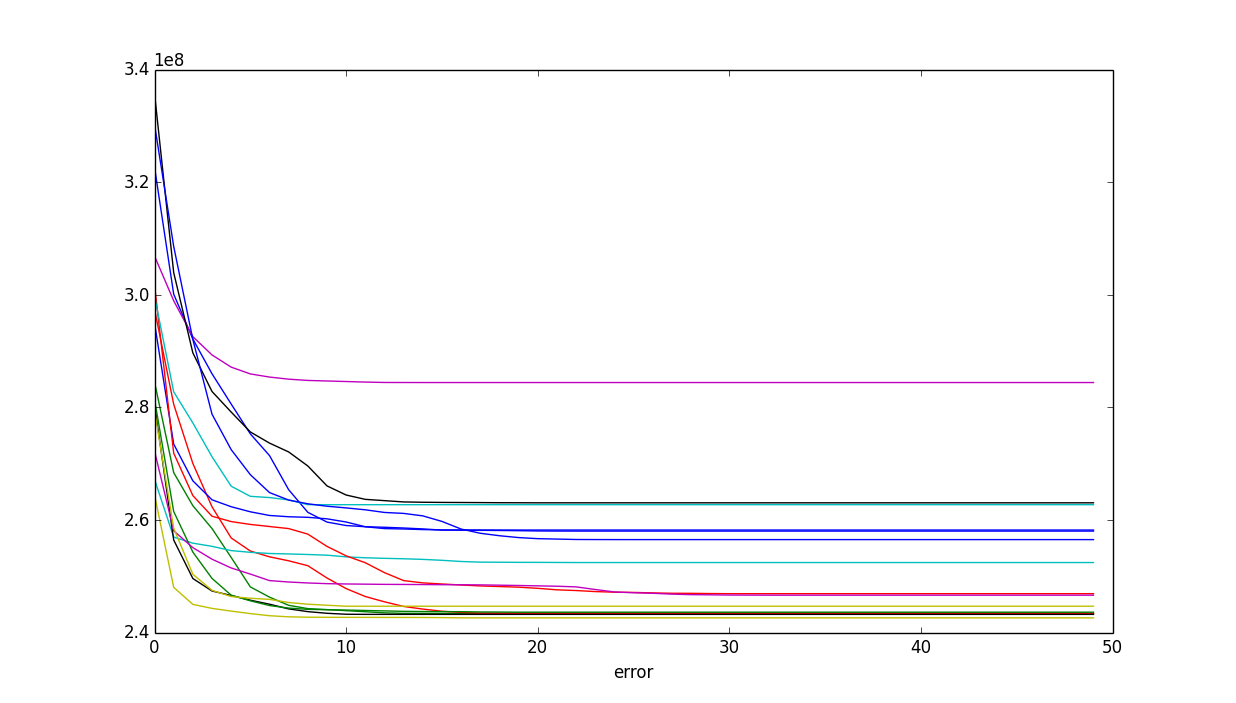
\includegraphics[width=100mm]{pic/q42.png}
\end{center}
\caption{The error over iteration of K-means}
\end{figure}

As we could see from the figure, all the 15 iterations converge within 50
iteration. For most instances, the alogrithm would converge within 15 $\sim$ 20
iterations.



\section{Collaboration}
I did not collaborate with classmates in this assignment. However, I refered to
some code online to finish my K-means algorithms. The link is:
https://github.com/stuntgoat/kmeans.git

Basically, I used the general code structure, the update and assign function.
I implemented my own data read and error plot function. Besides, I change the
interface of the general kmeans function for stop conditions. I also implement
the error function to get the error in each iteration for each cluster.





\end{document}
